\documentclass{standalone}
\usepackage{tikz}
\usetikzlibrary{patterns, positioning}


\begin{document}
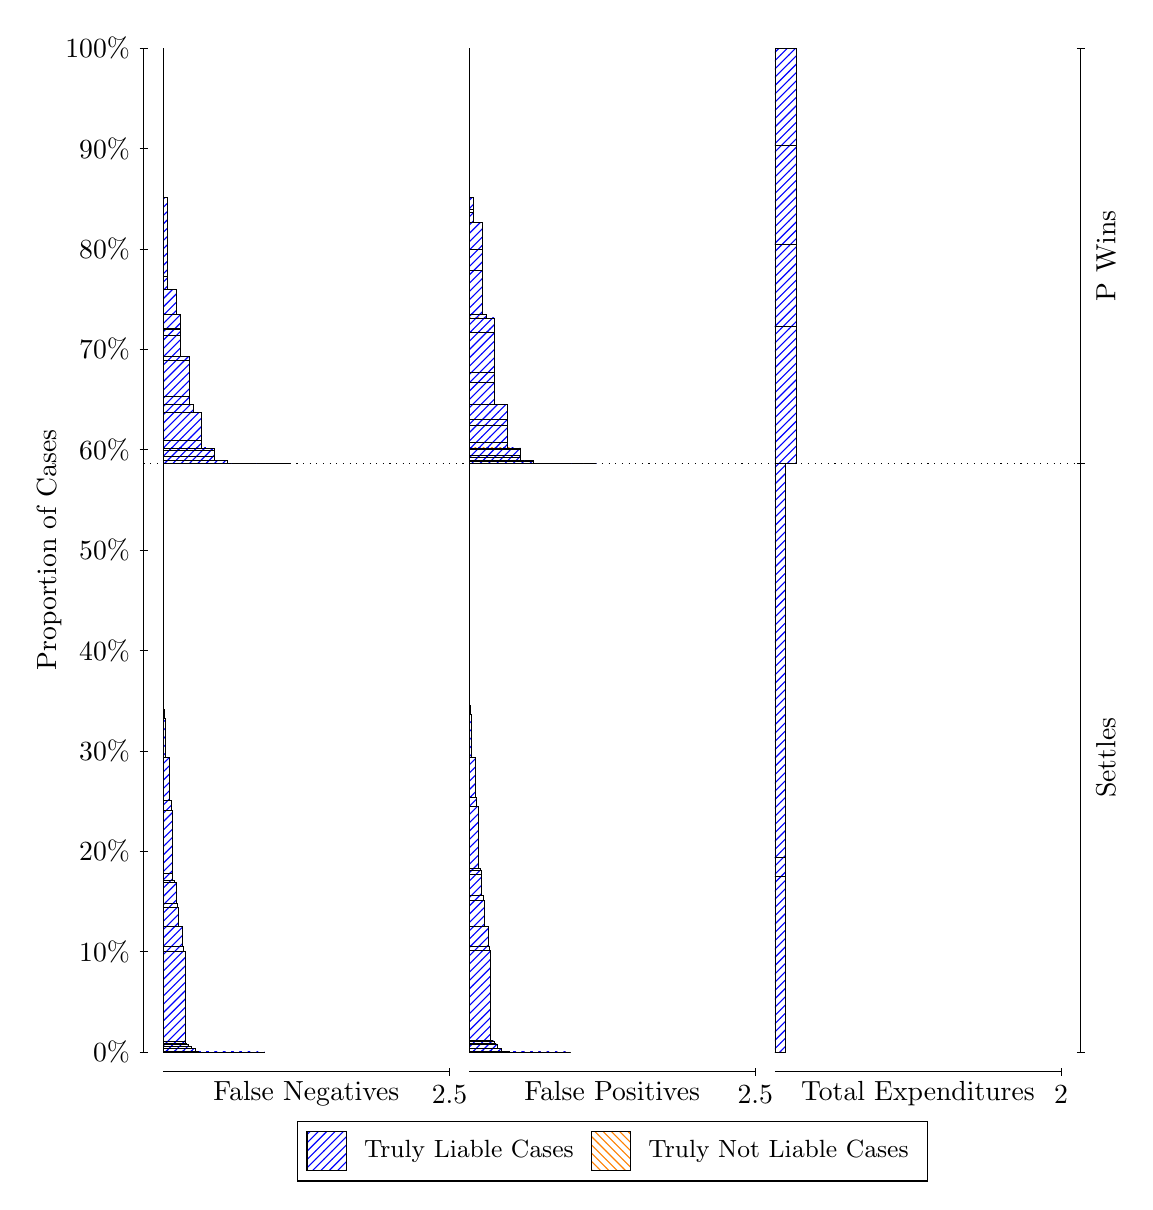
\begin{tikzpicture}
\draw[black, very thin] (1.5,1.75) -- (1.5,14.5);
\node[rotate=90, text=black, anchor=center] at (0.3, 8.125) {Proportion of Cases};
\draw[black, very thin] (1.45,1.75) -- (1.55,1.75);
\node[text=black, anchor=east] at (1.45, 1.75) {0\%};
\draw[black, very thin] (1.45,3.025) -- (1.55,3.025);
\node[text=black, anchor=east] at (1.45, 3.025) {10\%};
\draw[black, very thin] (1.45,4.3) -- (1.55,4.3);
\node[text=black, anchor=east] at (1.45, 4.3) {20\%};
\draw[black, very thin] (1.45,5.575) -- (1.55,5.575);
\node[text=black, anchor=east] at (1.45, 5.575) {30\%};
\draw[black, very thin] (1.45,6.85) -- (1.55,6.85);
\node[text=black, anchor=east] at (1.45, 6.85) {40\%};
\draw[black, very thin] (1.45,8.125) -- (1.55,8.125);
\node[text=black, anchor=east] at (1.45, 8.125) {50\%};
\draw[black, very thin] (1.45,9.4) -- (1.55,9.4);
\node[text=black, anchor=east] at (1.45, 9.4) {60\%};
\draw[black, very thin] (1.45,10.675) -- (1.55,10.675);
\node[text=black, anchor=east] at (1.45, 10.675) {70\%};
\draw[black, very thin] (1.45,11.95) -- (1.55,11.95);
\node[text=black, anchor=east] at (1.45, 11.95) {80\%};
\draw[black, very thin] (1.45,13.225) -- (1.55,13.225);
\node[text=black, anchor=east] at (1.45, 13.225) {90\%};
\draw[black, very thin] (1.45,14.5) -- (1.55,14.5);
\node[text=black, anchor=east] at (1.45, 14.5) {100\%};

\draw[black, very thin] (13.4,1.75) -- (13.4,14.5);
\draw[black, very thin] (13.35,1.75) -- (13.45,1.75);
\node[anchor=west] at (13.35, 1.75) {};
\draw[black, very thin] (13.35,9.224) -- (13.45,9.224);
\node[anchor=west] at (13.35, 9.224) {};
\draw[black, very thin] (13.35,14.5) -- (13.45,14.5);
\node[anchor=west] at (13.35, 14.5) {};

\draw[black, very thin, pattern color=blue, pattern=north east lines] (1.75,1.75) rectangle (3.0398,1.75);
\draw[black, very thin, pattern color=blue, pattern=north east lines] (1.75,1.75) rectangle (2.8945,1.75);
\draw[black, very thin, pattern color=blue, pattern=north east lines] (1.75,1.75) rectangle (2.8784,1.75);
\draw[black, very thin, pattern color=blue, pattern=north east lines] (1.75,1.75) rectangle (2.8218,1.75);
\draw[black, very thin, pattern color=blue, pattern=north east lines] (1.75,1.75) rectangle (2.7492,1.75);
\draw[black, very thin, pattern color=blue, pattern=north east lines] (1.75,1.75) rectangle (2.733,1.75);
\draw[black, very thin, pattern color=blue, pattern=north east lines] (1.75,1.75) rectangle (2.7169,1.75);
\draw[black, very thin, pattern color=blue, pattern=north east lines] (1.75,1.75) rectangle (2.6765,1.75);
\draw[black, very thin, pattern color=blue, pattern=north east lines] (1.75,1.75) rectangle (2.6604,1.75);
\draw[black, very thin, pattern color=blue, pattern=north east lines] (1.75,1.75) rectangle (2.5877,1.75);
\draw[black, very thin, pattern color=blue, pattern=north east lines] (1.75,1.75) rectangle (2.5715,1.75);
\draw[black, very thin, pattern color=blue, pattern=north east lines] (1.75,1.75) rectangle (2.5554,1.75);
\draw[black, very thin, pattern color=blue, pattern=north east lines] (1.75,1.75) rectangle (2.5312,1.75);
\draw[black, very thin, pattern color=blue, pattern=north east lines] (1.75,1.75) rectangle (2.515,1.75);
\draw[black, very thin, pattern color=blue, pattern=north east lines] (1.75,1.75) rectangle (2.4989,1.75);
\draw[black, very thin, pattern color=blue, pattern=north east lines] (1.75,1.75) rectangle (2.4262,1.75);
\draw[black, very thin, pattern color=blue, pattern=north east lines] (1.75,1.75) rectangle (2.4101,1.75);
\draw[black, very thin, pattern color=blue, pattern=north east lines] (1.75,1.75) rectangle (2.3939,1.75);
\draw[black, very thin, pattern color=blue, pattern=north east lines] (1.75,1.75) rectangle (2.3858,1.75);
\draw[black, very thin, pattern color=blue, pattern=north east lines] (1.75,1.75) rectangle (2.3697,1.75);
\draw[black, very thin, pattern color=blue, pattern=north east lines] (1.75,1.75) rectangle (2.3535,1.75);
\draw[black, very thin, pattern color=blue, pattern=north east lines] (1.75,1.75) rectangle (2.3374,1.75);
\draw[black, very thin, pattern color=blue, pattern=north east lines] (1.75,1.75) rectangle (2.3132,1.7511);
\draw[black, very thin, pattern color=blue, pattern=north east lines] (1.75,1.7511) rectangle (2.2647,1.7517);
\draw[black, very thin, pattern color=blue, pattern=north east lines] (1.75,1.7517) rectangle (2.2486,1.7517);
\draw[black, very thin, pattern color=blue, pattern=north east lines] (1.75,1.7517) rectangle (2.2324,1.7523);
\draw[black, very thin, pattern color=blue, pattern=north east lines] (1.75,1.7523) rectangle (2.2244,1.7523);
\draw[black, very thin, pattern color=blue, pattern=north east lines] (1.75,1.7523) rectangle (2.2082,1.7525);
\draw[black, very thin, pattern color=blue, pattern=north east lines] (1.75,1.7525) rectangle (2.1921,1.7544);
\draw[black, very thin, pattern color=blue, pattern=north east lines] (1.75,1.7544) rectangle (2.1759,1.7545);
\draw[black, very thin, pattern color=blue, pattern=north east lines] (1.75,1.7545) rectangle (2.1678,1.7648);
\draw[black, very thin, pattern color=blue, pattern=north east lines] (1.75,1.7648) rectangle (2.1517,1.7944);
\draw[black, very thin, pattern color=blue, pattern=north east lines] (1.75,1.7944) rectangle (2.1032,1.8201);
\draw[black, very thin, pattern color=blue, pattern=north east lines] (1.75,1.8201) rectangle (2.0871,1.825);
\draw[black, very thin, pattern color=blue, pattern=north east lines] (1.75,1.825) rectangle (2.0709,1.8512);
\draw[black, very thin, pattern color=blue, pattern=north east lines] (1.75,1.8512) rectangle (2.0629,1.8513);
\draw[black, very thin, pattern color=blue, pattern=north east lines] (1.75,1.8513) rectangle (2.0467,1.8562);
\draw[black, very thin, pattern color=blue, pattern=north east lines] (1.75,1.8562) rectangle (2.0306,1.8888);
\draw[black, very thin, pattern color=blue, pattern=north east lines] (1.75,1.8888) rectangle (2.0225,3.0303);
\draw[black, very thin, pattern color=blue, pattern=north east lines] (1.75,3.0303) rectangle (2.0144,3.0322);
\draw[black, very thin, pattern color=blue, pattern=north east lines] (1.75,3.0322) rectangle (2.0064,3.0933);
\draw[black, very thin, pattern color=blue, pattern=north east lines] (1.75,3.0933) rectangle (1.9902,3.342);
\draw[black, very thin, pattern color=blue, pattern=north east lines] (1.75,3.342) rectangle (1.9418,3.5827);
\draw[black, very thin, pattern color=blue, pattern=north east lines] (1.75,3.5827) rectangle (1.9256,3.6358);
\draw[black, very thin, pattern color=blue, pattern=north east lines] (1.75,3.6358) rectangle (1.9095,3.9032);
\draw[black, very thin, pattern color=blue, pattern=north east lines] (1.75,3.9032) rectangle (1.9014,3.9038);
\draw[black, very thin, pattern color=blue, pattern=north east lines] (1.75,3.9038) rectangle (1.8852,3.9295);
\draw[black, very thin, pattern color=blue, pattern=north east lines] (1.75,3.9295) rectangle (1.8691,4.0232);
\draw[black, very thin, pattern color=blue, pattern=north east lines] (1.75,4.0232) rectangle (1.861,4.8155);
\draw[black, very thin, pattern color=blue, pattern=north east lines] (1.75,4.8155) rectangle (1.8529,4.8207);
\draw[black, very thin, pattern color=blue, pattern=north east lines] (1.75,4.8207) rectangle (1.8449,4.941);
\draw[black, very thin, pattern color=blue, pattern=north east lines] (1.75,4.941) rectangle (1.8287,5.487);
\draw[black, very thin, pattern color=blue, pattern=north east lines] (1.75,5.487) rectangle (1.7803,5.9847);
\draw[black, very thin, pattern color=blue, pattern=north east lines] (1.75,5.9847) rectangle (1.7641,6.1027);
\draw[black, very thin, pattern color=orange, pattern=north west lines] (1.75,6.1027) rectangle (1.75,6.1027);
\draw[black, very thin, pattern color=blue, pattern=north east lines] (1.75,6.1027) rectangle (1.75,9.224);
\draw[black, very thin, pattern color=blue, pattern=north east lines] (1.75,9.224) rectangle (3.3668,9.224);
\draw[black, very thin, pattern color=blue, pattern=north east lines] (1.75,9.224) rectangle (3.2054,9.224);
\draw[black, very thin, pattern color=blue, pattern=north east lines] (1.75,9.224) rectangle (3.0439,9.224);
\draw[black, very thin, pattern color=blue, pattern=north east lines] (1.75,9.224) rectangle (2.9349,9.224);
\draw[black, very thin, pattern color=blue, pattern=north east lines] (1.75,9.224) rectangle (2.8824,9.2241);
\draw[black, very thin, pattern color=blue, pattern=north east lines] (1.75,9.2241) rectangle (2.8824,9.2242);
\draw[black, very thin, pattern color=blue, pattern=north east lines] (1.75,9.2242) rectangle (2.7734,9.2242);
\draw[black, very thin, pattern color=blue, pattern=north east lines] (1.75,9.2242) rectangle (2.7209,9.2263);
\draw[black, very thin, pattern color=blue, pattern=north east lines] (1.75,9.2263) rectangle (2.7209,9.2277);
\draw[black, very thin, pattern color=blue, pattern=north east lines] (1.75,9.2277) rectangle (2.6119,9.2277);
\draw[black, very thin, pattern color=blue, pattern=north east lines] (1.75,9.2277) rectangle (2.6119,9.2277);
\draw[black, very thin, pattern color=blue, pattern=north east lines] (1.75,9.2277) rectangle (2.5594,9.2587);
\draw[black, very thin, pattern color=blue, pattern=north east lines] (1.75,9.2587) rectangle (2.4504,9.2587);
\draw[black, very thin, pattern color=blue, pattern=north east lines] (1.75,9.2587) rectangle (2.4504,9.2588);
\draw[black, very thin, pattern color=blue, pattern=north east lines] (1.75,9.2588) rectangle (2.3979,9.3159);
\draw[black, very thin, pattern color=blue, pattern=north east lines] (1.75,9.3159) rectangle (2.3979,9.397);
\draw[black, very thin, pattern color=blue, pattern=north east lines] (1.75,9.397) rectangle (2.3979,9.4143);
\draw[black, very thin, pattern color=blue, pattern=north east lines] (1.75,9.4143) rectangle (2.2889,9.4223);
\draw[black, very thin, pattern color=blue, pattern=north east lines] (1.75,9.4223) rectangle (2.2889,9.4223);
\draw[black, very thin, pattern color=blue, pattern=north east lines] (1.75,9.4223) rectangle (2.2889,9.4227);
\draw[black, very thin, pattern color=blue, pattern=north east lines] (1.75,9.4227) rectangle (2.2365,9.5161);
\draw[black, very thin, pattern color=blue, pattern=north east lines] (1.75,9.5161) rectangle (2.2365,9.8727);
\draw[black, very thin, pattern color=blue, pattern=north east lines] (1.75,9.8727) rectangle (2.1275,9.8735);
\draw[black, very thin, pattern color=blue, pattern=north east lines] (1.75,9.8735) rectangle (2.1275,9.9755);
\draw[black, very thin, pattern color=blue, pattern=north east lines] (1.75,9.9755) rectangle (2.075,10.077);
\draw[black, very thin, pattern color=blue, pattern=north east lines] (1.75,10.077) rectangle (2.075,10.535);
\draw[black, very thin, pattern color=blue, pattern=north east lines] (1.75,10.535) rectangle (2.075,10.588);
\draw[black, very thin, pattern color=blue, pattern=north east lines] (1.75,10.588) rectangle (1.966,10.847);
\draw[black, very thin, pattern color=blue, pattern=north east lines] (1.75,10.847) rectangle (1.966,10.926);
\draw[black, very thin, pattern color=blue, pattern=north east lines] (1.75,10.926) rectangle (1.966,10.943);
\draw[black, very thin, pattern color=blue, pattern=north east lines] (1.75,10.943) rectangle (1.966,11.125);
\draw[black, very thin, pattern color=blue, pattern=north east lines] (1.75,11.125) rectangle (1.9135,11.438);
\draw[black, very thin, pattern color=blue, pattern=north east lines] (1.75,11.438) rectangle (1.8045,11.606);
\draw[black, very thin, pattern color=blue, pattern=north east lines] (1.75,11.606) rectangle (1.8045,12.599);
\draw[black, very thin, pattern color=blue, pattern=north east lines] (1.75,12.599) rectangle (1.752,12.651);
\draw[black, very thin, pattern color=blue, pattern=north east lines] (1.75,12.651) rectangle (1.752,12.651);
\draw[black, very thin, pattern color=orange, pattern=north west lines] (1.75,12.651) rectangle (1.75,12.651);
\draw[black, very thin, pattern color=blue, pattern=north east lines] (1.75,12.651) rectangle (1.75,14.5);
\draw[black, very thin, pattern color=orange, pattern=north west lines] (5.6333,1.75) rectangle (6.9232,1.75);
\draw[black, very thin, pattern color=blue, pattern=north east lines] (5.6333,1.75) rectangle (6.9232,1.75);
\draw[black, very thin, pattern color=orange, pattern=north west lines] (5.6333,1.75) rectangle (6.7778,1.75);
\draw[black, very thin, pattern color=blue, pattern=north east lines] (5.6333,1.75) rectangle (6.7778,1.75);
\draw[black, very thin, pattern color=blue, pattern=north east lines] (5.6333,1.75) rectangle (6.7617,1.75);
\draw[black, very thin, pattern color=orange, pattern=north west lines] (5.6333,1.75) rectangle (6.6325,1.75);
\draw[black, very thin, pattern color=blue, pattern=north east lines] (5.6333,1.75) rectangle (6.6325,1.75);
\draw[black, very thin, pattern color=blue, pattern=north east lines] (5.6333,1.75) rectangle (6.6164,1.75);
\draw[black, very thin, pattern color=blue, pattern=north east lines] (5.6333,1.75) rectangle (6.6002,1.75);
\draw[black, very thin, pattern color=orange, pattern=north west lines] (5.6333,1.75) rectangle (6.5598,1.75);
\draw[black, very thin, pattern color=blue, pattern=north east lines] (5.6333,1.75) rectangle (6.5598,1.75);
\draw[black, very thin, pattern color=blue, pattern=north east lines] (5.6333,1.75) rectangle (6.471,1.75);
\draw[black, very thin, pattern color=blue, pattern=north east lines] (5.6333,1.75) rectangle (6.4549,1.75);
\draw[black, very thin, pattern color=blue, pattern=north east lines] (5.6333,1.75) rectangle (6.4387,1.75);
\draw[black, very thin, pattern color=orange, pattern=north west lines] (5.6333,1.75) rectangle (6.4145,1.75);
\draw[black, very thin, pattern color=blue, pattern=north east lines] (5.6333,1.75) rectangle (6.4145,1.75);
\draw[black, very thin, pattern color=blue, pattern=north east lines] (5.6333,1.75) rectangle (6.3984,1.75);
\draw[black, very thin, pattern color=blue, pattern=north east lines] (5.6333,1.75) rectangle (6.3095,1.75);
\draw[black, very thin, pattern color=blue, pattern=north east lines] (5.6333,1.75) rectangle (6.2934,1.75);
\draw[black, very thin, pattern color=blue, pattern=north east lines] (5.6333,1.75) rectangle (6.2772,1.75);
\draw[black, very thin, pattern color=orange, pattern=north west lines] (5.6333,1.75) rectangle (6.2692,1.75);
\draw[black, very thin, pattern color=blue, pattern=north east lines] (5.6333,1.75) rectangle (6.2692,1.75);
\draw[black, very thin, pattern color=blue, pattern=north east lines] (5.6333,1.75) rectangle (6.253,1.75);
\draw[black, very thin, pattern color=blue, pattern=north east lines] (5.6333,1.75) rectangle (6.2369,1.75);
\draw[black, very thin, pattern color=orange, pattern=north west lines] (5.6333,1.75) rectangle (6.1965,1.75);
\draw[black, very thin, pattern color=blue, pattern=north east lines] (5.6333,1.75) rectangle (6.1965,1.7511);
\draw[black, very thin, pattern color=blue, pattern=north east lines] (5.6333,1.7511) rectangle (6.1481,1.7536);
\draw[black, very thin, pattern color=blue, pattern=north east lines] (5.6333,1.7536) rectangle (6.1319,1.7538);
\draw[black, very thin, pattern color=orange, pattern=north west lines] (5.6333,1.7538) rectangle (6.1238,1.7538);
\draw[black, very thin, pattern color=blue, pattern=north east lines] (5.6333,1.7538) rectangle (6.1238,1.7538);
\draw[black, very thin, pattern color=blue, pattern=north east lines] (5.6333,1.7538) rectangle (6.1158,1.7543);
\draw[black, very thin, pattern color=blue, pattern=north east lines] (5.6333,1.7543) rectangle (6.1077,1.7544);
\draw[black, very thin, pattern color=blue, pattern=north east lines] (5.6333,1.7544) rectangle (6.0915,1.7546);
\draw[black, very thin, pattern color=blue, pattern=north east lines] (5.6333,1.7546) rectangle (6.0754,1.7546);
\draw[black, very thin, pattern color=orange, pattern=north west lines] (5.6333,1.7546) rectangle (6.0512,1.7546);
\draw[black, very thin, pattern color=blue, pattern=north east lines] (5.6333,1.7546) rectangle (6.0512,1.7649);
\draw[black, very thin, pattern color=blue, pattern=north east lines] (5.6333,1.7649) rectangle (6.035,1.7944);
\draw[black, very thin, pattern color=blue, pattern=north east lines] (5.6333,1.7944) rectangle (5.9866,1.8526);
\draw[black, very thin, pattern color=blue, pattern=north east lines] (5.6333,1.8526) rectangle (5.9704,1.8594);
\draw[black, very thin, pattern color=blue, pattern=north east lines] (5.6333,1.8594) rectangle (5.9624,1.8596);
\draw[black, very thin, pattern color=blue, pattern=north east lines] (5.6333,1.8596) rectangle (5.9543,1.8858);
\draw[black, very thin, pattern color=blue, pattern=north east lines] (5.6333,1.8858) rectangle (5.9462,1.8907);
\draw[black, very thin, pattern color=blue, pattern=north east lines] (5.6333,1.8907) rectangle (5.9301,1.8957);
\draw[black, very thin, pattern color=blue, pattern=north east lines] (5.6333,1.8957) rectangle (5.9139,1.8958);
\draw[black, very thin, pattern color=orange, pattern=north west lines] (5.6333,1.8958) rectangle (5.9058,1.8958);
\draw[black, very thin, pattern color=blue, pattern=north east lines] (5.6333,1.8958) rectangle (5.9058,3.0372);
\draw[black, very thin, pattern color=blue, pattern=north east lines] (5.6333,3.0372) rectangle (5.8897,3.0981);
\draw[black, very thin, pattern color=blue, pattern=north east lines] (5.6333,3.0981) rectangle (5.8735,3.3419);
\draw[black, very thin, pattern color=blue, pattern=north east lines] (5.6333,3.3419) rectangle (5.8251,3.6759);
\draw[black, very thin, pattern color=blue, pattern=north east lines] (5.6333,3.6759) rectangle (5.8089,3.7341);
\draw[black, very thin, pattern color=blue, pattern=north east lines] (5.6333,3.7341) rectangle (5.8009,3.7364);
\draw[black, very thin, pattern color=blue, pattern=north east lines] (5.6333,3.7364) rectangle (5.7928,4.0039);
\draw[black, very thin, pattern color=blue, pattern=north east lines] (5.6333,4.0039) rectangle (5.7847,4.0527);
\draw[black, very thin, pattern color=blue, pattern=north east lines] (5.6333,4.0527) rectangle (5.7686,4.0783);
\draw[black, very thin, pattern color=blue, pattern=north east lines] (5.6333,4.0783) rectangle (5.7524,4.0789);
\draw[black, very thin, pattern color=blue, pattern=north east lines] (5.6333,4.0789) rectangle (5.7444,4.8712);
\draw[black, very thin, pattern color=blue, pattern=north east lines] (5.6333,4.8712) rectangle (5.7282,4.9892);
\draw[black, very thin, pattern color=blue, pattern=north east lines] (5.6333,4.9892) rectangle (5.7121,5.487);
\draw[black, very thin, pattern color=blue, pattern=north east lines] (5.6333,5.487) rectangle (5.6636,6.033);
\draw[black, very thin, pattern color=blue, pattern=north east lines] (5.6333,6.033) rectangle (5.6475,6.1533);
\draw[black, very thin, pattern color=blue, pattern=north east lines] (5.6333,6.1533) rectangle (5.6394,6.1584);
\draw[black, very thin, pattern color=blue, pattern=north east lines] (5.6333,6.1584) rectangle (5.6333,9.224);
\draw[black, very thin, pattern color=orange, pattern=north west lines] (5.6333,9.224) rectangle (7.2502,9.224);
\draw[black, very thin, pattern color=blue, pattern=north east lines] (5.6333,9.224) rectangle (7.2502,9.224);
\draw[black, very thin, pattern color=orange, pattern=north west lines] (5.6333,9.224) rectangle (7.0887,9.224);
\draw[black, very thin, pattern color=blue, pattern=north east lines] (5.6333,9.224) rectangle (7.0887,9.224);
\draw[black, very thin, pattern color=blue, pattern=north east lines] (5.6333,9.224) rectangle (6.9272,9.224);
\draw[black, very thin, pattern color=orange, pattern=north west lines] (5.6333,9.224) rectangle (6.9272,9.224);
\draw[black, very thin, pattern color=blue, pattern=north east lines] (5.6333,9.224) rectangle (6.9272,9.224);
\draw[black, very thin, pattern color=blue, pattern=north east lines] (5.6333,9.224) rectangle (6.7657,9.224);
\draw[black, very thin, pattern color=blue, pattern=north east lines] (5.6333,9.224) rectangle (6.7657,9.2241);
\draw[black, very thin, pattern color=orange, pattern=north west lines] (5.6333,9.2241) rectangle (6.7657,9.2241);
\draw[black, very thin, pattern color=blue, pattern=north east lines] (5.6333,9.2241) rectangle (6.7657,9.2242);
\draw[black, very thin, pattern color=orange, pattern=north west lines] (5.6333,9.2242) rectangle (6.6042,9.2242);
\draw[black, very thin, pattern color=blue, pattern=north east lines] (5.6333,9.2242) rectangle (6.6042,9.2263);
\draw[black, very thin, pattern color=blue, pattern=north east lines] (5.6333,9.2263) rectangle (6.6042,9.2271);
\draw[black, very thin, pattern color=blue, pattern=north east lines] (5.6333,9.2271) rectangle (6.6042,9.2277);
\draw[black, very thin, pattern color=orange, pattern=north west lines] (5.6333,9.2277) rectangle (6.4952,9.2277);
\draw[black, very thin, pattern color=blue, pattern=north east lines] (5.6333,9.2277) rectangle (6.4952,9.2277);
\draw[black, very thin, pattern color=orange, pattern=north west lines] (5.6333,9.2277) rectangle (6.4428,9.2277);
\draw[black, very thin, pattern color=blue, pattern=north east lines] (5.6333,9.2277) rectangle (6.4428,9.2531);
\draw[black, very thin, pattern color=blue, pattern=north east lines] (5.6333,9.2531) rectangle (6.4428,9.2588);
\draw[black, very thin, pattern color=blue, pattern=north east lines] (5.6333,9.2588) rectangle (6.3338,9.2588);
\draw[black, very thin, pattern color=orange, pattern=north west lines] (5.6333,9.2588) rectangle (6.3338,9.2588);
\draw[black, very thin, pattern color=blue, pattern=north east lines] (5.6333,9.2588) rectangle (6.3338,9.2588);
\draw[black, very thin, pattern color=blue, pattern=north east lines] (5.6333,9.2588) rectangle (6.2813,9.3086);
\draw[black, very thin, pattern color=blue, pattern=north east lines] (5.6333,9.3086) rectangle (6.2813,9.3263);
\draw[black, very thin, pattern color=orange, pattern=north west lines] (5.6333,9.3263) rectangle (6.2813,9.3263);
\draw[black, very thin, pattern color=blue, pattern=north east lines] (5.6333,9.3263) rectangle (6.2813,9.3982);
\draw[black, very thin, pattern color=blue, pattern=north east lines] (5.6333,9.3982) rectangle (6.2813,9.4227);
\draw[black, very thin, pattern color=blue, pattern=north east lines] (5.6333,9.4227) rectangle (6.1723,9.4227);
\draw[black, very thin, pattern color=orange, pattern=north west lines] (5.6333,9.4227) rectangle (6.1723,9.4227);
\draw[black, very thin, pattern color=blue, pattern=north east lines] (5.6333,9.4227) rectangle (6.1723,9.4227);
\draw[black, very thin, pattern color=blue, pattern=north east lines] (5.6333,9.4227) rectangle (6.1198,9.494);
\draw[black, very thin, pattern color=blue, pattern=north east lines] (5.6333,9.494) rectangle (6.1198,9.7138);
\draw[black, very thin, pattern color=orange, pattern=north west lines] (5.6333,9.7138) rectangle (6.1198,9.7138);
\draw[black, very thin, pattern color=blue, pattern=north east lines] (5.6333,9.7138) rectangle (6.1198,9.7868);
\draw[black, very thin, pattern color=blue, pattern=north east lines] (5.6333,9.7868) rectangle (6.1198,9.9754);
\draw[black, very thin, pattern color=blue, pattern=north east lines] (5.6333,9.9754) rectangle (6.0108,9.9754);
\draw[black, very thin, pattern color=orange, pattern=north west lines] (5.6333,9.9754) rectangle (6.0108,9.9754);
\draw[black, very thin, pattern color=blue, pattern=north east lines] (5.6333,9.9754) rectangle (6.0108,9.9755);
\draw[black, very thin, pattern color=blue, pattern=north east lines] (5.6333,9.9755) rectangle (5.9583,10.253);
\draw[black, very thin, pattern color=blue, pattern=north east lines] (5.6333,10.253) rectangle (5.9583,10.383);
\draw[black, very thin, pattern color=blue, pattern=north east lines] (5.6333,10.383) rectangle (5.9583,10.894);
\draw[black, very thin, pattern color=blue, pattern=north east lines] (5.6333,10.894) rectangle (5.9583,11.073);
\draw[black, very thin, pattern color=blue, pattern=north east lines] (5.6333,11.073) rectangle (5.8493,11.073);
\draw[black, very thin, pattern color=orange, pattern=north west lines] (5.6333,11.073) rectangle (5.8493,11.073);
\draw[black, very thin, pattern color=blue, pattern=north east lines] (5.6333,11.073) rectangle (5.8493,11.114);
\draw[black, very thin, pattern color=blue, pattern=north east lines] (5.6333,11.114) rectangle (5.8493,11.125);
\draw[black, very thin, pattern color=blue, pattern=north east lines] (5.6333,11.125) rectangle (5.7968,11.678);
\draw[black, very thin, pattern color=blue, pattern=north east lines] (5.6333,11.678) rectangle (5.7968,11.943);
\draw[black, very thin, pattern color=blue, pattern=north east lines] (5.6333,11.943) rectangle (5.7968,12.286);
\draw[black, very thin, pattern color=blue, pattern=north east lines] (5.6333,12.286) rectangle (5.6878,12.408);
\draw[black, very thin, pattern color=orange, pattern=north west lines] (5.6333,12.408) rectangle (5.6878,12.408);
\draw[black, very thin, pattern color=blue, pattern=north east lines] (5.6333,12.408) rectangle (5.6878,12.458);
\draw[black, very thin, pattern color=blue, pattern=north east lines] (5.6333,12.458) rectangle (5.6878,12.599);
\draw[black, very thin, pattern color=blue, pattern=north east lines] (5.6333,12.599) rectangle (5.6354,12.682);
\draw[black, very thin, pattern color=blue, pattern=north east lines] (5.6333,12.682) rectangle (5.6354,12.995);
\draw[black, very thin, pattern color=blue, pattern=north east lines] (5.6333,12.995) rectangle (5.6354,13.136);
\draw[black, very thin, pattern color=blue, pattern=north east lines] (5.6333,13.136) rectangle (5.6333,14.5);
\draw[black, very thin, pattern color=orange, pattern=north west lines] (9.5167,1.75) rectangle (9.6529,1.75);
\draw[black, very thin, pattern color=blue, pattern=north east lines] (9.5167,1.75) rectangle (9.6529,3.978);
\draw[black, very thin, pattern color=orange, pattern=north west lines] (9.5167,3.978) rectangle (9.6529,3.978);
\draw[black, very thin, pattern color=blue, pattern=north east lines] (9.5167,3.978) rectangle (9.6529,4.2253);
\draw[black, very thin, pattern color=orange, pattern=north west lines] (9.5167,4.2253) rectangle (9.6529,4.2253);
\draw[black, very thin, pattern color=blue, pattern=north east lines] (9.5167,4.2253) rectangle (9.6529,9.224);
\draw[black, very thin, pattern color=orange, pattern=north west lines] (9.5167,9.224) rectangle (9.7892,9.224);
\draw[black, very thin, pattern color=blue, pattern=north east lines] (9.5167,9.224) rectangle (9.7892,10.962);
\draw[black, very thin, pattern color=orange, pattern=north west lines] (9.5167,10.962) rectangle (9.7892,10.962);
\draw[black, very thin, pattern color=blue, pattern=north east lines] (9.5167,10.962) rectangle (9.7892,12.008);
\draw[black, very thin, pattern color=orange, pattern=north west lines] (9.5167,12.008) rectangle (9.7892,12.008);
\draw[black, very thin, pattern color=blue, pattern=north east lines] (9.5167,12.008) rectangle (9.7892,13.265);
\draw[black, very thin, pattern color=orange, pattern=north west lines] (9.5167,13.265) rectangle (9.7892,13.265);
\draw[black, very thin, pattern color=blue, pattern=north east lines] (9.5167,13.265) rectangle (9.7892,14.5);
\draw[black, dotted] (1.5,9.224) -- (13.4,9.224);
\draw[black, very thin] (1.75,1.5) -- (5.3833,1.5);
\node[text=black, anchor=north] at (3.5667, 1.5) {False Negatives};
\draw[black, very thin] (5.3833,1.45) -- (5.3833,1.55);
\node[text=black, anchor=north] at (5.3833, 1.45) {2.5};

\draw[black, very thin] (5.6333,1.5) -- (9.2667,1.5);
\node[text=black, anchor=north] at (7.45, 1.5) {False Positives};
\draw[black, very thin] (9.2667,1.45) -- (9.2667,1.55);
\node[text=black, anchor=north] at (9.2667, 1.45) {2.5};

\draw[black, very thin] (9.5167,1.5) -- (13.15,1.5);
\node[text=black, anchor=north] at (11.333, 1.5) {Total Expenditures};
\draw[black, very thin] (13.15,1.45) -- (13.15,1.55);
\node[text=black, anchor=north] at (13.15, 1.45) {2};

\node[text=black, centered, rotate=90] at (13.72, 5.487) {Settles};
\node[text=black, centered, rotate=90] at (13.72, 11.862) {P Wins};

\draw (7.449999999999999,1.5) node[draw=none] (baseCoordinate) {};
\begin{scope}[align=center]
        \matrix[scale=0.5, draw=black, below=0.5cm of baseCoordinate, nodes={draw}, column sep=0.1cm]{
            \node[rectangle, draw, minimum width=0.5cm, minimum height=0.5cm, pattern color=blue, pattern=north east lines] {}; &
            \node[draw=none, font=\small, text=black] (B) {Truly Liable Cases}; &
            \node[rectangle, draw, minimum width=0.5cm, minimum height=0.5cm, pattern color=orange, pattern=north west lines] {}; &
            \node[draw=none, font=\small, text=black] (B) {Truly Not Liable Cases}; \\
            };
\end{scope}

\end{tikzpicture}
\end{document}